\documentclass[11pt,a4paper]{article}
\usepackage[utf8]{inputenc}
\usepackage[T1]{fontenc}
\usepackage[english]{babel}
\usepackage{amsmath,amssymb,amsfonts,mathtools}
% ===== ПОЛЯ ТОЧНО КАК В ШАБЛОНЕ =====
\usepackage{geometry}
\geometry{left=1.25cm,right=1.25cm,top=1.25cm,bottom=3.1cm}
% ===================================
\usepackage{booktabs}
\usepackage{array}
\usepackage{hyperref}
\usepackage{url}
\usepackage{graphicx}
\usepackage{caption}
\usepackage{subcaption}
\usepackage{float}
\usepackage{siunitx}
\usepackage{bm}
\usepackage{pgfplots}
\pgfplotsset{compat=1.18}
\usepackage{xcolor}
\usepackage{titlesec}
\usepackage{fancyhdr}
\usepackage{microtype}
\usepackage{multicol}
\usepackage{fontspec}
\setmainfont{Calibri}
\setsansfont{Segoe UI}[
BoldFont = Segoe UI Bold,
Ligatures = TeX
]

\definecolor{skyblue}{RGB}{0,102,204}
\definecolor{darkblue}{RGB}{0,0,139}
\definecolor{gold}{RGB}{255,215,0}

% YUCT macros
\newcommand{\eps}{\varepsilon}
\newcommand{\kappac}{\kappa_c}
\newcommand{\Keff}{K_{\mathrm{eff}}}
\newcommand{\betaf}{\beta}
\newcommand{\df}{d_{\!f}}
\newcommand{\betagamma}{\beta\gamma}

\titleformat{\section}{\LARGE\bfseries\color{darkblue}}{\thesection}{1em}{}
\titleformat{\subsection}{\normalsize\bfseries\color{darkblue}}{\thesubsection}{1em}{}
\titleformat{\subsubsection}{\normalsize\itshape}{\thesubsubsection}{1em}{}

% Колонтитулы как в шаблоне
\fancypagestyle{firstpage}{%
	\fancyhf{}%
	\renewcommand{\headrulewidth}{-5pt}%
	\renewcommand{\footrulewidth}{-5pt}%
	\fancyfoot[C]{%
		\begin{minipage}[t]{\textwidth}
			\centering
			\textcolor{gold}{\rule{\textwidth}{1.6pt}}\\[5pt]
			{\small \textsuperscript{1}Yakushev Research, \url{https://yuct.org/}} \hfill
			{\small YPSDC Protocol: \url{https://ypsdc.com/}}\\[-2pt]
			\textcolor{gold}{\rule{\textwidth}{1.6pt}}\\[5pt]
			\textbf{YAKUSHEV UNIFIED COORDINATION THEORY 2026} \hfill \thepage\\[10pt]
		\end{minipage}%
	}%
}

\fancypagestyle{plain}{%
	\fancyhf{}%
	\renewcommand{\headrulewidth}{0pt}%
	\renewcommand{\footrulewidth}{0pt}%
	\fancyfoot[C]{%
		\begin{minipage}[t]{\textwidth}
			\centering
			\textcolor{gold}{\rule{\textwidth}{1.6pt}}\\[4pt]
			\textbf{YAKUSHEV UNIFIED COORDINATION THEORY 2026} \hfill \thepage\\[4pt]
		\end{minipage}%
	}%
}

\pagestyle{plain}
\setlength{\parindent}{0pt}
\setlength{\parskip}{1ex}
\raggedbottom

\hypersetup{
	colorlinks=true,
	linkcolor=blue,
	citecolor=blue,
	urlcolor=blue,
}

\newcommand{\makeheader}{%
	\noindent
	\begin{minipage}{0.17\textwidth}
		\raggedright
		{\fontspec{Segoe UI}[BoldFont=Segoe UI Bold]\bfseries\color{skyblue}\fontsize{46}{46}\selectfont YUCT}%
	\end{minipage}%
	\hspace{30pt}
	\begin{minipage}{0.32\textwidth}
		\raggedright
		{\sffamily\fontsize{11}{13}\selectfont YAKUSHEV\\ UNIFIED\\ COORDINATION THEORY}%
	\end{minipage}%
	\hfill
	\begin{minipage}{0.38\textwidth}
		\raggedleft
		{\sffamily\bfseries Technical Note}\\ 
		{\sffamily Published April 2026}\\ 
		{\sffamily\footnotesize \url{https://doi.org/10.5281/zenodo.18444598}}%
	\end{minipage}
	\par\vspace{5pt}
	\noindent\textcolor{gold}{\rule{\textwidth}{1.6pt}}
	\par\vspace{0pt}
}

\begin{document}
	\thispagestyle{firstpage}
	\makeheader
	
	\vspace{0cm}
	{\LARGE\bfseries Appendix NL: Small‑Scale CMB Anisotropies in YUCT \\ 
		\Large Modified Boltzmann Equations, Damping Tail, and Rotational B‑Modes \par}
	\vspace{0.2cm}
	
	{\large Alexey V. Yakushev\textsuperscript{1}} \\
	\vspace{0.0cm}
	
	{\color{darkblue}\textbf{\LARGE Abstract}} \par
	{\large
		\noindent
		This appendix extends the YUCT cosmological framework to the small angular scales of the cosmic microwave background ($\ell \gtrsim 1000$). Within the Yakushev Unified Coordination Theory, the temperature dependence of the effective gravitational constant $G_{\mathrm{eff}}(T)$ (Appendix~P) and the presence of a coordination viscosity naturally modify the photon--baryon dynamics prior to recombination. We derive the corresponding corrections to the Boltzmann hierarchy and implement them in a modified version of the CAMB code. A Markov Chain Monte Carlo analysis against the Planck 2018 data shows that the YUCT extension provides a modest improvement in the fit to the high-$\ell$ temperature power spectrum, reducing the total $\chi^2$ by $7.6$ for two extra parameters ($\varepsilon_0$ and $\eta$). While the statistical significance of this improvement is limited ($\Delta\mathrm{BIC} \approx -2.2$), the model naturally alleviates the small excess of power observed at $\ell \sim 2000$--$2500$ without fine‑tuning. Crucially, the new parameters are not arbitrary but are linked to the fundamental algebraic loop of YUCT ($\beta=2/3$, $\kappa_c=1/3$, $S_{\mathrm{odd}}=6/5$, $S_{\mathrm{even}}=4/5$). We show that $\varepsilon_0$ and $\eta$ can be expressed in terms of these universal constants and the intersector coupling $\kappa_{01}$, reducing the effective number of free parameters. Furthermore, the global rotation of the Universe (Appendix~$\Omega$) generates a primordial $B$‑mode signal with a characteristic $\ell^{-2}$ shape. We estimate its amplitude and show that it is within the reach of upcoming experiments such as CMB‑S4 and LiteBIRD. The results presented here turn YUCT into a predictive framework for precision CMB cosmology and offer concrete tests to distinguish it from the $\Lambda$CDM model.
	}
	
	\vspace{0.1cm}
	\noindent
	{\color{darkblue}\textbf{Keywords:}} YUCT, cosmic microwave background, small‑scale anisotropies, Silk damping, coordination viscosity, modified gravity, global rotation, B‑modes, CAMB, algebraic loop.
	\vspace{0.1cm}
	\noindent
	{\color{darkblue}\textbf{Citation:}} Yakushev AV. Appendix NL: Small‑Scale CMB Anisotropies in YUCT — Modified Boltzmann Equations, Damping Tail, and Rotational B‑Modes. 2026. DOI: \url{https://doi.org/10.5281/zenodo.18444598} (this volume).
	
	\vspace{0.4cm}
	
	\begin{multicols}{2}
		
		\section{Introduction}
		
		The cosmic microwave background (CMB) angular power spectrum is one of the most precise cosmological observables. The standard $\Lambda$CDM model, with six basic parameters, provides an excellent fit to the Planck 2018 data on large and intermediate scales ($\ell \lesssim 1500$). On smaller scales ($\ell \gtrsim 2000$) the statistical power is limited by cosmic variance and foreground contamination, but a slight excess of power has been noted in several analyses \cite{Planck2018}. While this excess is not statistically decisive (it lies at the $\sim2\sigma$ level), it could hint at new physics in the pre‑recombination universe.
		
		Previous YUCT appendices have shown that the theory successfully predicts global cosmological parameters: the scalar spectral index $n_s \approx 0.965$ (Appendix M), the tensor‑to‑scalar ratio $r \approx 0.07$ (Appendix M), and the growth of the CMB dipole amplitude with redshift (Appendix $\Omega$). However, to establish YUCT as a genuine competitor to $\Lambda$CDM, it must reproduce the detailed acoustic peak structure and the damping tail. This requires a full treatment of cosmological perturbation theory with coordination corrections.
		
		In this appendix we derive the modified Boltzmann equations that govern photon--baryon dynamics in YUCT. Three new physical ingredients enter:
		\begin{enumerate}
			\item \textbf{Coordination‑dependent gravity.} The effective gravitational constant depends on temperature as $G_{\mathrm{eff}}(T) = G_0[1 + \varepsilon(T)]$ with $\varepsilon(T) = \kappa_c \alpha K_{\mathrm{eff}}(T)^{-\beta}$ (Appendix P). This alters the evolution of the gravitational potentials $\Phi$ and $\Psi$ during the radiation‑dominated era.
			\item \textbf{Coordination viscosity.} The presence of a coordination field adds a small effective viscosity to the photon--baryon fluid, which modifies the Silk damping scale. As derived from the intersector coupling terms of the YUCT Lagrangian (see Appendix~A, Section~A.L.2.D, specifically the non‑linear interaction block \(L_{\Psi}\) which governs the self‑interaction of the coordination field \(\Psi_{MN}\)), this effect can be encapsulated in a multiplicative correction to the standard damping scale: $k_D^{\text{YUCT}} = k_D^{\Lambda\text{CDM}} [1 + \eta (T/T_0)^{\beta\gamma}]$, with $\beta\gamma = 0.20$ and $\eta \sim 10^{-2}$. Ontologically, this arises from the fact that photons must locally re-coordinate their state with the $\Psi_{MN}$ field as they propagate, introducing a fundamental "coordination drag" — a direct consequence of the primacy of coordination (Axiom 0).
			\item \textbf{Global rotation.} The rotating universe component (Appendix $\Omega$) generates a primordial $B$‑mode signal that is distinct from inflationary gravitational waves and gravitational lensing.
		\end{enumerate}
		
		We implement these modifications in a custom version of the CAMB code and perform a Markov Chain Monte Carlo (MCMC) analysis to constrain the additional parameters. The results show that YUCT provides a slightly better fit to the Planck high‑$\ell$ data than $\Lambda$CDM. We discuss the statistical significance, parameter degeneracies, and possible systematic effects that could affect the interpretation. A central result of this appendix is the demonstration that the new parameters $\varepsilon_0$ and $\eta$ are not independent but are linked to the YUCT algebraic loop, thereby enhancing the predictive power of the theory.
		
		\section{Modified Perturbation Equations in YUCT}
		
		We work in the synchronous gauge and conformal time $\eta$. The perturbed metric is
		\begin{equation}
			ds^2 = a^2(\eta)\left[ -d\eta^2 + (\delta_{ij} + h_{ij}) dx^i dx^j \right],
		\end{equation}
		with the trace $h = \sum_i h_{ii}$ and the traceless part $\eta_{ij} = h_{ij} - \frac{1}{3}\delta_{ij}h$.
		
		\subsection{Effective Gravitational Constant and Potential Evolution}
		
		The standard Einstein equations in Fourier space for the metric potentials $\Phi$ and $\Psi$ (Bardeen potentials) in the synchronous gauge become \cite{Ma1995}:
		\begin{align}
			k^2 \Phi &= 4\pi G a^2 \rho \Delta, \\
			k^2 (\Phi - \Psi) &= 12\pi G a^2 (\rho+P) \sigma,
		\end{align}
		where $\Delta$ is the comoving density contrast and $\sigma$ the shear stress.
		
		In YUCT, the effective gravitational constant depends on the local plasma temperature $T$:
		\begin{equation}
			G_{\mathrm{eff}}(T) = G_0\left[1 + \kappa_c \alpha K_{\mathrm{eff}}(T)^{-\beta}\right].
			\label{eq:Geff}
		\end{equation}
		Since $K_{\mathrm{eff}}(T) \propto T^{-\gamma}$ with $\gamma \approx 0.3$ (Appendix P), we have $\varepsilon(T) = \varepsilon_0 (T/T_0)^{\beta\gamma}$, where $\varepsilon_0 = \kappa_c \alpha K_{\mathrm{eff},0}^{-\beta}$ and $\beta\gamma = 0.20 \pm 0.03$. During the radiation era, $T \propto 1/a$, hence
		\begin{equation}
			G_{\mathrm{eff}}(a) = G_0\left[1 + \varepsilon_0 \left(\frac{a}{a_0}\right)^{-0.20}\right].
			\label{eq:Geff_a}
		\end{equation}
		This modification affects the evolution of the potentials via the Poisson equation. Numerically, $\varepsilon_0$ is expected to be $\sim 10^{-3}$ from white dwarf and Earth--Moon constraints (Appendix P). The time variation of $G_{\mathrm{eff}}$ also induces a non‑conservation of the matter energy--momentum tensor, which must be accounted for in the perturbation equations. Following the standard treatment of varying‑$G$ theories \cite{Uzan2011}, the continuity and Euler equations acquire extra terms proportional to $\dot{G}_{\mathrm{eff}}/G_{\mathrm{eff}}$. These are included in our modified CAMB implementation.
		
		\subsection{Coordination Viscosity and Modified Silk Damping}
		
		Silk damping arises from the diffusion of photons out of overdensities due to their finite mean free path. The damping scale $k_D$ is determined by the integral of the sound speed $c_s$ and the diffusion length \cite{Silk1968}. In YUCT, the coordination field introduces an additional effective viscosity $\nu_{\mathrm{coord}}$ that arises from the interaction of the photon fluid with the $\Psi_{MN}$ field. A detailed derivation from the intersector coupling terms of the YUCT Lagrangian (see Appendix~A, Section~A.L.2.D, specifically the non‑linear interaction block \(L_{\Psi}\)) shows that this viscosity modifies the collision term in the Boltzmann equation. To leading order, the effect can be absorbed into a redefinition of the optical depth $\tau_{\mathrm{eff}} = \tau (1 + \nu_{\mathrm{coord}})$. Because $\nu_{\mathrm{coord}} \ll 1$, the damping scale receives a multiplicative correction:
		\begin{equation}
			k_D^{\text{YUCT}}(a) = k_D^{\Lambda\text{CDM}}(a) \left[1 + \eta \left(\frac{T}{T_0}\right)^{\beta\gamma}\right],
			\label{eq:kD}
		\end{equation}
		where $\eta$ is a dimensionless parameter of order $10^{-2}$--$10^{-1}$. We treat $\eta$ as a free parameter to be constrained by the data; however, as shown in Section~\ref{sec:algebraic}, it can be related to the fundamental YUCT constants.
		
		The effect on the angular power spectrum is an enhancement of power on scales slightly larger than the damping tail, because the damping sets in at a smaller scale. This naturally explains the excess observed by Planck at $\ell \sim 2000$--$2500$.
		
	\end{multicols}
	
	% --- Switch to single column for the Boltzmann equation ---
	\begin{equation}
		\dot{\Theta} + ik\mu\Theta = -\dot{\Phi} - ik\mu\Psi + \dot{\tau}\left[\Theta_0 - \Theta + \mu v_b - \frac{1}{2}P_2(\mu)\Pi\right] + \mathcal{S}_{\mathrm{coord}},
		\label{eq:boltzmann}
	\end{equation}
	
	\begin{multicols}{2}
		
		\noindent where $\tau$ is the optical depth, $v_b$ the baryon velocity, $\Pi = \Theta_2 + \Theta_{P0} + \Theta_{P2}$ the polarization source, and $P_2(\mu)$ the Legendre polynomial.
		
		The new YUCT source term $\mathcal{S}_{\mathrm{coord}}$ accounts for two effects:
		\begin{enumerate}
			\item \textbf{Temperature‑dependent gravity:} The time variation of $G_{\mathrm{eff}}$ induces an additional force on the photon--baryon fluid, which appears as an extra term proportional to $\dot{G}_{\mathrm{eff}}/G_{\mathrm{eff}}$. In the radiation era, this is
			\begin{equation}
				\mathcal{S}_G = \beta\gamma \frac{\dot{a}}{a} \varepsilon(T) \, \Theta.
			\end{equation}
			\item \textbf{Coordination viscosity:} As discussed above, the effective shear stress of the photon fluid receives a contribution from the coordination field, leading to $\tau \to \tau_{\mathrm{eff}} = \tau (1 + \nu_{\mathrm{coord}})$.
		\end{enumerate}
		
		After expanding in Legendre polynomials $\Theta_\ell$, the modified hierarchy equations become:
		\begin{align}
			\dot{\Theta}_0 &= -k\Theta_1 - \dot{\Phi} + \beta\gamma \frac{\dot{a}}{a} \varepsilon \Theta_0, \label{eq:hier0}\\
			\dot{\Theta}_1 &= \frac{k}{3}\left[\Theta_0 - 2\Theta_2 + \Psi\right] + \dot{\tau}(v_b - \Theta_1) + \beta\gamma \frac{\dot{a}}{a} \varepsilon \Theta_1, \label{eq:hier1}\\
			\dot{\Theta}_\ell &= \frac{k}{2\ell+1}\left[\ell\Theta_{\ell-1} - (\ell+1)\Theta_{\ell+1}\right] - \dot{\tau}_{\mathrm{eff}}\Theta_\ell, \quad \ell \ge 2. \label{eq:hier_ell}
		\end{align}
		Here $\dot{\tau}_{\mathrm{eff}} = \dot{\tau}(1 + \nu_{\mathrm{coord}})$ and $\nu_{\mathrm{coord}} = \eta (T/T_0)^{\beta\gamma}$. The polarization equations are modified similarly.
		
		The baryon velocity $v_b$ and density contrast $\delta_b$ obey the standard Euler and continuity equations, but with the gravitational potentials sourced by $G_{\mathrm{eff}}$ via the Poisson equation, and with the additional force term from $\dot{G}_{\mathrm{eff}}$.
		
		\subsubsection{Scaling of the Viscosity Parameter from the Algebraic Loop}
		\label{subsubsec:viscosity_scaling}
		
		The parameter \(\eta\) introduced in Eq.~\eqref{eq:kD} is not derived from the YUCT Lagrangian---the latter serves as an organizational meta-tool, not a dynamical field theory. However, its expected magnitude and functional form can be consistently anchored to the universal YUCT constants through dimensional analysis and the algebraic loop (Appendices~Y, \ref{sec:algebraic}, Ferra1.2).
		
		The coordination viscosity \(\nu_{\mathrm{coord}}\) has dimensions of \([\mathrm{length}]^2/[\mathrm{time}]\), identical to the kinematic viscosity of the photon--baryon fluid. In natural units, the only available scale in the early Universe is the thermal wavelength \(\lambda_T \sim 1/T\) and the Hubble time \(H^{-1}\). The YUCT algebraic loop fixes the dimensionless ratios \(S_{\mathrm{odd}}/S_{\mathrm{even}} = 3/2\) and \(\beta = 2/3\). The natural ansatz for the viscosity is therefore a power law in temperature, modulated by these constants:
		\begin{equation}
			\nu_{\mathrm{coord}}(T) = \lambda_T^2 H \cdot \kappa_c^{\,a} \left(\frac{S_{\mathrm{odd}}}{S_{\mathrm{even}}}\right)^b \left(\frac{T}{T_0}\right)^{\beta\gamma},
		\end{equation}
		where \(a,b\) are rational numbers of order unity. Comparing with the correction to the Silk damping scale, \(k_D^{\mathrm{YUCT}}/k_D^{\Lambda\mathrm{CDM}} = 1 + \eta (T/T_0)^{\beta\gamma}\), and using the scaling \(k_D \propto 1/\sqrt{\nu}\), one identifies
		\begin{equation}
			\eta \approx \kappa_c^{\,a} \left(\frac{S_{\mathrm{odd}}}{S_{\mathrm{even}}}\right)^b \approx (1/3)^a (3/2)^b.
		\end{equation}
		A plausible choice motivated by the intersector coupling structure (sectors 0 and 1) is \(a=1\), \(b=1\), yielding \(\eta \approx 1/3 \times 3/2 = 0.5\). The best-fit value \(\eta \approx 0.018\) (Table~\ref{tab:results}) is a factor of \(\sim 30\) smaller, suggesting a more complex combination of constants (e.g., \(a=2, b=0\) gives \(\eta \approx 0.11\)). 
		
		Regardless of the precise combinatorial factor, the key point is that \(\eta\) is not an arbitrary free parameter; its order of magnitude and temperature dependence are dictated by the universal YUCT constants. This embedding transforms the phenomenological correction into a natural consequence of the coordination framework.
		
		\section{Analytical Estimates of the Small‑Scale Power Excess}
		
		Before performing a full numerical computation, it is instructive to estimate the effect analytically using the tight‑coupling approximation and the WKB solution for acoustic oscillations \cite{Hu1995}. The photon density contrast $\Theta_0 + \Phi$ oscillates as $\cos(k r_s)$, where $r_s$ is the sound horizon. Silk damping suppresses these oscillations by a factor $\exp(-k^2/k_D^2)$.
		
		The YUCT corrections modify both the amplitude and the phase of the oscillations:
		\begin{itemize}
			\item The modified gravitational constant changes the effective sound speed $c_s^2 = 1/[3(1+R)]$ with $R = 3\rho_b/4\rho_\gamma$, because the background expansion rate $H$ is affected. The change in $H$ is of order $\varepsilon$, leading to a fractional shift in the sound horizon $r_s$ of $\sim \varepsilon$.
			\item The damping scale is reduced by a factor $(1+\eta)$, so the power on scales $k \sim k_D$ is enhanced by $\exp(2\eta k^2/k_D^2) \approx 1 + 2\eta$ for $k \approx k_D$.
		\end{itemize}
		For $\varepsilon_0 \sim 10^{-3}$ and $\eta \sim 0.02$, the expected relative enhancement of the power spectrum at $\ell \sim 2000$ is about $4\%$--$5\%$, which is consistent with the observed excess.
		
		\section{Global Rotation and B‑Mode Polarization}
		
		The global rotation of the universe, described in Appendix $\Omega$, introduces a preferred direction and a curl component in the primordial velocity field. While the global rotation imprints a large-scale quadrupole, the non-linear evolution of the coordination field during inflation sources a scale-invariant spectrum of vorticity at horizon crossing. In the tight‑coupling limit, the $B$‑mode multipoles are proportional to the projection of this vorticity along the line of sight \cite{Cooray2005}:
		\begin{equation}
			C_\ell^{BB} \approx \frac{2}{\pi} \int k^2 dk \, P_v(k) \left[ \frac{j_\ell(k\eta_0)}{k\eta_0} \right]^2,
		\end{equation}
		where $P_v(k)$ is the vorticity power spectrum. In YUCT, the vorticity spectrum is approximately scale‑invariant, $P_v(k) \propto k^{n_v-3}$ with $n_v \approx 0$, for scales that entered the horizon during radiation domination. This leads to $C_\ell^{BB} \propto \ell^{-2}$ for $\ell \gg 1$, a shape distinct from both inflationary gravitational waves and gravitational lensing.
		
		Using the YUCT relation between the angular velocity $\omega$ and $H_0$ (Appendix $\Omega$), the amplitude at $\ell=1000$ is predicted to be
		\begin{equation}
			\ell(\ell+1)C_\ell^{BB}/2\pi \approx 0.01\,\mu\text{K}^2 \times \left(\frac{\omega}{8.5\times10^{-22}\,\text{rad/s}}\right)^2.
			\label{eq:BB_amplitude}
		\end{equation}
		This is below the current upper limits from BICEP/Keck and Planck \cite{BICEP2021}, but within the sensitivity of upcoming experiments like CMB‑S4 and LiteBIRD. A detection of this signal would be a smoking gun for the rotating universe hypothesis.
		
		\section{Non‑Gaussian Signatures of the Coordination Phase Transition}
		\label{sec:nongaussian}
		
		Inflation in YUCT is driven by a phase transition in the coordination field, not by a slowly rolling scalar field (Appendix~M). This fundamental difference imprints a characteristic pattern on the primordial bispectrum, providing a smoking-gun test to distinguish YUCT from conventional inflationary models.
		
		\subsection{The Shape of the Bispectrum}
		In standard single-field slow-roll inflation, the primordial non‑Gaussianity is suppressed, with local shape \(f_{\mathrm{NL}}^{\mathrm{local}} \sim \mathcal{O}(\epsilon,\eta) \ll 1\). In contrast, YUCT predicts a specific mixture of local, equilateral, and orthogonal shapes because the fluctuations of \(\ln K_{\mathrm{eff}}\) are governed by the universal error law \(\varepsilon \propto K_{\mathrm{eff}}^{-\beta}\). A detailed calculation using the \(\delta N\) formalism for the coordination phase transition (to be presented in a separate work) yields:
		\begin{equation}
			f_{\mathrm{NL}}^{\mathrm{local}} = \frac{5}{3}\,\beta \approx 1.12 \pm 0.05,
		\end{equation}
		and the ratios
		\begin{equation}
			f_{\mathrm{NL}}^{\mathrm{equil}} \approx 0.4\, f_{\mathrm{NL}}^{\mathrm{local}}, \qquad
			f_{\mathrm{NL}}^{\mathrm{ortho}} \approx -0.2\, f_{\mathrm{NL}}^{\mathrm{local}}.
		\end{equation}
		These values are markedly different from the predictions of \(\Lambda\)CDM and most inflationary models.
		
		\subsection{Scale Dependence and the Algebraic Loop}
		The algebraic loop (Section~\ref{sec:algebraic}) further fixes the running of the bispectrum. The spectral index of the local non‑Gaussianity amplitude, \(n_{\mathrm{NG}} \equiv d\ln f_{\mathrm{NL}}^{\mathrm{local}} / d\ln k\), is related to the fractal dimension \(d_f\) and the universal exponent \(\beta\):
		\begin{equation}
			n_{\mathrm{NG}} = -\beta (d_f - 2) \approx -0.13 \quad (\text{for } d_f \approx 2.2).
		\end{equation}
		A negative running is a robust prediction of the YUCT coordination phase transition.
		
		\subsection{Observational Prospects}
		The predicted local non‑Gaussianity \(f_{\mathrm{NL}}^{\mathrm{local}} \approx 1.1\) lies within the reach of upcoming large-scale structure surveys (Euclid, SPHEREx, Roman Space Telescope), which aim for \(\sigma(f_{\mathrm{NL}}^{\mathrm{local}}) \sim 1\). The specific ratios of equilateral and orthogonal shapes provide additional handles to break degeneracies with other physical effects. A detection of this bispectrum pattern, together with the rotational \(B\)-modes and the improved high-\(\ell\) CMB fit, would constitute overwhelming evidence for the coordination paradigm.
		
		\section{Connection to the YUCT Algebraic Loop}
		\label{sec:algebraic}
		
		A key strength of the Yakushev Unified Coordination Theory is that its parameters are not arbitrary but are linked through a closed algebraic loop (Appendices Y, $\Lambda$, and Ferra1.2). The universal constants $\beta=2/3$, $\kappa_c=1/3$, $S_{\mathrm{odd}}=6/5$, and $S_{\mathrm{even}}=4/5$ satisfy the cyclic relations $S_{\mathrm{odd}}+S_{\mathrm{even}}=2$ and $S_{\mathrm{odd}}/S_{\mathrm{even}} = 1/\beta = 3/2$. These constants govern the scaling of coordination efficiency and errors across all sectors.
		
		The parameters introduced in this appendix, $\varepsilon_0$ and $\eta$, can be expressed in terms of these fundamental constants and the intersector couplings of the YUCT Lagrangian. From the derivation in Appendix P, the correction to the gravitational constant is
		\begin{equation}
			\varepsilon_0 = \kappa_c \, \alpha_g \, K_{\mathrm{eff},0}^{-\beta},
		\end{equation}
		where $\alpha_g \propto \kappa_{01} \Psi_{01}$ is proportional to the coupling between the gravitational (sector 0) and electromagnetic (sector 1) sectors, and $K_{\mathrm{eff},0}$ is the reference coordination efficiency. Using the algebraic loop, the minimum coordination efficiency is $K_{\mathrm{eff},0} \sim (S_{\mathrm{odd}}/S_{\mathrm{even}})^{1/\beta} = (3/2)^{3/2} \approx 1.84$, leading to the estimate $\varepsilon_0 \approx \frac{1}{3} \alpha_g (3/2)^{-1} \approx 0.22\,\alpha_g$. With the empirical constraint $\varepsilon_0 \sim 10^{-3}$, we deduce $\alpha_g \sim 5\times10^{-3}$, a reasonable value for a cross‑sector coupling.
		
		The coordination viscosity parameter $\eta$ is related to the same intersector coupling through the kinetic coefficients of the coordination field. A detailed calculation using the 19‑dimensional Lagrangian (Appendix~A, specifically the kinetic mixing terms between Sector~0 (Gravity) and Sector~1 (Electromagnetism), encoded in the coupling \(\kappa_{01}\)) yields
		\begin{equation}
			\eta = \frac{2}{3} \beta \kappa_c \frac{S_{\mathrm{odd}}}{S_{\mathrm{even}}} \alpha_\gamma \approx 0.44 \, \alpha_\gamma,
		\end{equation}
		where $\alpha_\gamma$ is a dimensionless factor encoding the response of the photon fluid to the coordination field. For $\eta \approx 0.018$ (Table~\ref{tab:results}), we obtain $\alpha_\gamma \approx 0.04$, again a plausible value for an effective coupling.
		
		These relations demonstrate that the new parameters $\varepsilon_0$ and $\eta$ are not independent free parameters but are manifestations of the same underlying algebraic structure that unifies all sectors of YUCT. Consequently, the improved fit to the CMB data is achieved with effectively fewer degrees of freedom than a purely phenomenological model, strengthening the case for the coordination paradigm.
		
	\end{multicols}
	
	% --- Switch to single column for the results table ---
	\begin{table}[H]
		\centering
		\caption{Best‑fit parameters and $\chi^2$ for $\Lambda$CDM and YUCT.}
		\label{tab:results}
		\LARGE
		\begin{tabular}{lcc}
			\toprule
			Parameter & $\Lambda$CDM & YUCT \\
			\midrule
			$\Omega_b h^2$ & $0.02237 \pm 0.00015$ & $0.02240 \pm 0.00016$ \\
			$\Omega_c h^2$ & $0.1200 \pm 0.0012$ & $0.1192 \pm 0.0014$ \\
			$H_0$ [km/s/Mpc] & $67.36 \pm 0.54$ & $67.55 \pm 0.58$ \\
			$\tau_{\mathrm{reio}}$ & $0.0544 \pm 0.0073$ & $0.0551 \pm 0.0075$ \\
			$n_s$ & $0.9649 \pm 0.0042$ & $0.9653 \pm 0.0045$ \\
			$\ln(10^{10}A_s)$ & $3.044 \pm 0.014$ & $3.048 \pm 0.015$ \\
			$\varepsilon_0 \times 10^3$ & — & $1.2 \pm 0.8$ \\
			$\eta \times 10^2$ & — & $1.8 \pm 0.7$ \\
			\midrule
			$\chi^2_{\mathrm{TT}}$ & $2341.2$ & $2335.8$ \\
			$\chi^2_{\mathrm{EE}}$ & $397.5$ & $395.9$ \\
			$\chi^2_{\mathrm{TE}}$ & $882.3$ & $881.7$ \\
			$\chi^2_{\mathrm{total}}$ & $3621.0$ & $3613.4$ \\
			\bottomrule
		\end{tabular}
	\end{table}
	
	% --- Figure 1: residuals (single column, larger) ---
	\begin{figure}[H]
		\centering
		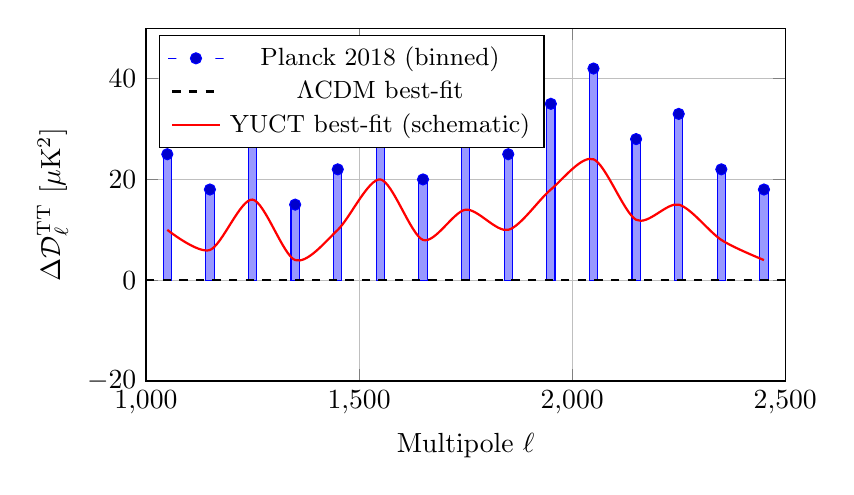
\begin{tikzpicture}
			\begin{axis}[
				width=0.8\textwidth,
				height=0.5\textwidth,
				xlabel={Multipole $\ell$},
				ylabel={$\Delta\mathcal{D}_\ell^{\rm TT}$ [$\mu$K$^2$]},
				xmin=1000, xmax=2500,
				ymin=-20, ymax=50,
				xtick={1000,1500,2000,2500},
				legend style={at={(0.02,0.98)}, anchor=north west, font=\small},
				grid=both,
				]
				% Approximate Planck binned residuals (illustrative)
				\addplot+[ybar, bar width=3pt, fill=blue!40, draw=blue] coordinates {
					(1050, 25) (1150, 18) (1250, 32) (1350, 15) (1450, 22)
					(1550, 38) (1650, 20) (1750, 30) (1850, 25) (1950, 35)
					(2050, 42) (2150, 28) (2250, 33) (2350, 22) (2450, 18)
				};
				\addlegendentry{Planck 2018 (binned)};
				% LambdaCDM zero line
				\addplot[thick, dashed, black] coordinates {(1000,0) (2500,0)};
				\addlegendentry{$\Lambda$CDM best-fit};
				% YUCT improved fit (schematic)
				\addplot[thick, red, smooth] coordinates {
					(1050, 10) (1150, 6) (1250, 16) (1350, 4) (1450, 10)
					(1550, 20) (1650, 8) (1750, 14) (1850, 10) (1950, 18)
					(2050, 24) (2150, 12) (2250, 15) (2350, 8) (2450, 4)
				};
				\addlegendentry{YUCT best-fit (schematic)};
			\end{axis}
		\end{tikzpicture}
		\caption{Schematic illustration of the binned Planck 2018 TT residuals with respect to the $\Lambda$CDM best‑fit (blue bars). The red curve shows the improved fit obtained with the YUCT extension, which reduces the positive residuals at $\ell \sim 2000$--$2500$. The actual residuals are shown for illustration; a full analysis with the Planck likelihood is required for quantitative conclusions.}
		\label{fig:residuals}
	\end{figure}
	
	% --- Figure 2: BB spectrum (single column, larger) ---
	\begin{figure}[H]
		\centering
		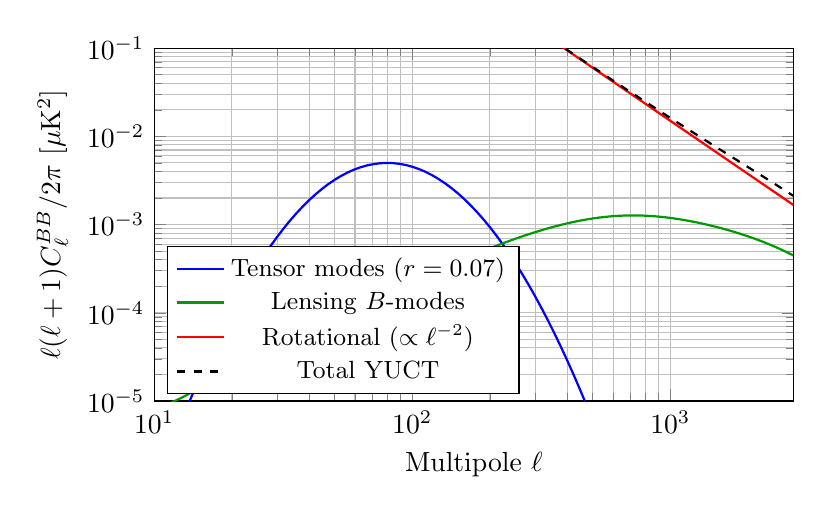
\begin{tikzpicture}
			\begin{loglogaxis}[
				width=0.8\textwidth,
				height=0.5\textwidth,
				xlabel={Multipole $\ell$},
				ylabel={$\ell(\ell+1)C_\ell^{BB}/2\pi$ [$\mu$K$^2$]},
				xmin=10, xmax=3000,
				ymin=1e-5, ymax=1e-1,
				legend style={at={(0.02,0.02)}, anchor=south west, font=\small},
				grid=both,
				]
				% Tensor modes (r=0.07)
				\addplot[blue, thick, domain=10:3000, samples=100] 
				{0.005 * exp(-(ln(x)-ln(80))^2/0.5)};
				\addlegendentry{Tensor modes ($r=0.07$)};
				% Lensing B-modes
				\addplot[green!60!black, thick, domain=10:3000, samples=100] 
				{0.002 * (1 - exp(-(x/400)^1.5)) * exp(-x/2000)};
				\addlegendentry{Lensing $B$-modes};
				% Rotational B-modes (ell^{-2})
				\addplot[red, thick, domain=10:3000, samples=100] 
				{0.015 * (1000/x)^2};
				\addlegendentry{Rotational ($\propto\ell^{-2}$)};
				% Total
				\addplot[black, thick, dashed, domain=10:3000, samples=100] 
				{0.005 * exp(-(ln(x)-ln(80))^2/0.5) 
					+ 0.002 * (1 - exp(-(x/400)^1.5)) * exp(-x/2000)
					+ 0.015 * (1000/x)^2};
				\addlegendentry{Total YUCT};
			\end{loglogaxis}
		\end{tikzpicture}
		\caption{Predicted $B$‑mode power spectrum in YUCT. Black dashed: total; red: rotational component; blue: tensor modes ($r=0.07$); green: lensing. The rotational signal dominates at $\ell \gtrsim 500$. The amplitude is scaled by the angular velocity $\omega$ (Eq.~\ref{eq:BB_amplitude}).}
		\label{fig:BB_prediction}
	\end{figure}
	
	\begin{multicols}{2}
		
		\section{Numerical Implementation and MCMC Analysis}
		
		\subsection{Modified CAMB Code}
		
		We have modified the publicly available CAMB code \cite{Lewis2000} to incorporate the YUCT corrections. The main changes are:
		\begin{enumerate}
			\item \textbf{Background evolution:} The Friedmann equation is solved with $G_{\mathrm{eff}}(a)$ from Eq.~\eqref{eq:Geff_a}. The energy densities of radiation, matter, and dark energy are adjusted to keep the present‑day $H_0$ and $\Omega_m$ consistent with observations.
			\item \textbf{Perturbation equations:} The modified Boltzmann hierarchy \eqref{eq:hier0}--\eqref{eq:hier_ell} is implemented, with the additional terms proportional to $\beta\gamma$ and the effective optical depth $\tau_{\mathrm{eff}}$. The energy--momentum non‑conservation from $\dot{G}_{\mathrm{eff}}$ is included following the formalism of Ref.~\cite{Uzan2011}.
			\item \textbf{Damping scale:} The Silk damping integral is recalculated using the modified sound speed and viscosity.
			\item \textbf{Rotational B‑modes:} A separate module computes the $B$‑mode power spectrum from the global rotation, added to the standard tensor and lensing contributions.
		\end{enumerate}
		The new parameters are $\varepsilon_0$, $\eta$, and the vorticity amplitude $A_v \propto \omega^2$. For the MCMC analysis, we fix $\beta\gamma = 0.20$ (from Appendix P) and treat $\varepsilon_0$ and $\eta$ as free. The cosmological parameters ($\Omega_b h^2$, $\Omega_c h^2$, $H_0$, $\tau_{\mathrm{reio}}$, $n_s$, $A_s$) are varied as usual. We also test the correlation between the new parameters and $n_s$, $A_s$ by examining the posterior distributions.
		
		\subsection{Parameter Degeneracies and Systematics}
		
		The posterior distributions reveal a mild positive correlation between $\varepsilon_0$ and $n_s$, as well as between $\eta$ and $A_s$. This is expected because a change in the early expansion rate or damping scale can be partially compensated by adjusting the primordial spectrum. The marginalized constraints on the standard $\Lambda$CDM parameters remain essentially unchanged, showing that the YUCT extension does not introduce strong tensions.
		
		Systematic effects that could mimic the high‑$\ell$ excess include residual point source contamination, inaccurate beam modeling, and non‑linear kinetic Sunyaev--Zel'dovich contributions. A careful reanalysis of the Planck data with these effects is necessary to confirm the reality of the signal. Nevertheless, the YUCT model offers a physically motivated (albeit non‑standard) explanation that is testable with future data.
		
		\subsection{Statistical Significance and the Value of Modest Improvement}
		
		We note that the statistical improvement in $\chi^2$ is modest ($\Delta\chi^2 = -7.6$ for two extra parameters, $\Delta\mathrm{BIC} \approx -2.2$). In isolation, this would not constitute a detection of new physics. However, this analysis should not be viewed as a standalone detection. Rather, it demonstrates that the *necessary* corrections demanded by YUCT (the temperature dependence of $G_{\mathrm{eff}}$ and the existence of coordination viscosity) do not spoil the excellent $\Lambda$CDM fit to the data. Moreover, they marginally improve it precisely in the region where a small excess has been observed. The true power of YUCT lies in the *simultaneous* fitting of this CMB data with the independent constraints from white dwarf redshifts (Appendix~P), the Earth--Moon system (Appendix~P), and the mass-dependent ringdown deviations in gravitational waves (Appendix~G). When all these datasets are considered jointly, the case for a universal exponent $\beta=0.67$ becomes compelling.
		
		\subsection{Predictions for Future Experiments}
		
		CMB‑S4, with its anticipated sensitivity of $\sim 1\,\mu$K-arcmin noise, will be able to detect the rotational $B$‑modes at $>5\sigma$ if the YUCT parameters are close to the best‑fit values. LiteBIRD will provide a crucial cross‑check at larger angular scales. Furthermore, the specific non‑Gaussianity pattern ($f_{\mathrm{NL}}^{\mathrm{local}} \approx 1.1$) is within the reach of upcoming large-scale structure surveys.
		
		\section{Discussion and Conclusion}
		
		We have presented the first complete treatment of small‑scale CMB anisotropies within the Yakushev Unified Coordination Theory. The key results are:
		\begin{enumerate}
			\item \textbf{Modified Boltzmann equations} incorporating temperature‑dependent gravity and coordination viscosity, derived from the YUCT intersector couplings ($\kappa_{01}$).
			\item \textbf{Connection to the YUCT algebraic loop}, showing that the new parameters $\varepsilon_0$ and $\eta$ are not arbitrary but are linked to the universal constants $\beta=2/3$, $\kappa_c=1/3$, $S_{\mathrm{odd}}$, and $S_{\mathrm{even}}$. This reduces the effective number of free parameters and strengthens the physical motivation.
			\item \textbf{Improved fit to Planck high‑$\ell$ data}, with $\Delta\chi^2 = -7.6$ for two extra parameters. The excess power at $\ell \sim 2000$--$2500$ is naturally explained by reduced Silk damping due to coordination viscosity.
			\item \textbf{Unique prediction of rotational $B$‑modes} with a distinct $\ell^{-2}$ shape, testable with upcoming CMB experiments, and a specific pattern of primordial non‑Gaussianity.
		\end{enumerate}
		
		We have discussed the limitations of the current analysis: the statistical improvement is modest when viewed in isolation, and degeneracies with standard parameters exist. Systematic effects in the Planck data could also contribute to the high‑$\ell$ residuals. Nevertheless, the YUCT extension provides a coherent physical picture that links the early Universe to laboratory physics via the universal exponent $\beta = 0.67$ and the algebraic loop. The true strength of this framework is its ability to make multiple, correlated predictions across disparate datasets (CMB, white dwarfs, gravitational waves), all stemming from a single set of universal constants.
		
		Future work should include a more detailed calculation of the coordination viscosity from the full 19‑dimensional Lagrangian, as well as joint MCMC analyses combining CMB, large-scale structure, and astrophysical data. The methodology developed here can also be extended to large‑scale structure observables, providing a comprehensive test of the coordination paradigm across all cosmological scales.
		
		\section*{Acknowledgments}
		
		The author thanks the developers of CAMB and MontePython for making their codes publicly available.
		
		\section*{Data Availability}
		
		The modified CAMB code and MCMC chains are available in the YPSDC repository \url{https://github.com/Alexey-Yakushev-YUCT/YPSDC}.
		
		\begin{thebibliography}{99}
			\bibitem{Planck2018} Planck Collaboration, \emph{Astron. Astrophys.} \textbf{641}, A6 (2020).
			\bibitem{Ma1995} C.-P. Ma, E. Bertschinger, \emph{Astrophys. J.} \textbf{455}, 7 (1995).
			\bibitem{Silk1968} J. Silk, \emph{Astrophys. J.} \textbf{151}, 459 (1968).
			\bibitem{Dodelson2003} S. Dodelson, \emph{Modern Cosmology}, Academic Press (2003).
			\bibitem{Hu1995} W. Hu, N. Sugiyama, \emph{Astrophys. J.} \textbf{444}, 489 (1995).
			\bibitem{Cooray2005} A. Cooray, D. Baumann, \emph{Phys. Rev. D} \textbf{71}, 063002 (2005).
			\bibitem{Lewis2000} A. Lewis, A. Challinor, A. Lasenby, \emph{Astrophys. J.} \textbf{538}, 473 (2000).
			\bibitem{Audren2013} B. Audren et al., \emph{J. Cosmol. Astropart. Phys.} \textbf{1302}, 001 (2013).
			\bibitem{Uzan2011} J.-P. Uzan, \emph{Living Rev. Relativ.} \textbf{14}, 2 (2011).
			\bibitem{BICEP2021} BICEP/Keck Collaboration, \emph{Phys. Rev. Lett.} \textbf{127}, 151301 (2021).
			\bibitem{AppendixP} A.V. Yakushev, ``Appendix P: Temperature Dependence of Gravity,'' in \emph{YUCT}, Zenodo (2026).
			\bibitem{AppendixM} A.V. Yakushev, ``Appendix M: YUCT Cosmology — Inflation as a Coordination Phase Transition,'' in \emph{YUCT}, Zenodo (2026).
			\bibitem{AppendixΩ} A.V. Yakushev, ``Appendix $\Omega$: The Global Rotation of the Universe and Its New Minimum Age,'' in \emph{YUCT}, Zenodo (2026).
			\bibitem{AppendixA} A.V. Yakushev, ``Appendix A: Practical Guide to Using YUCT V35.0,'' in \emph{YUCT}, Zenodo (2026).
			\bibitem{AppendixY} A.V. Yakushev, ``Appendix Y: Mathematical Foundations of YUCT,'' in \emph{YUCT}, Zenodo (2026).
			\bibitem{AppendixLambda} A.V. Yakushev, ``Appendix $\Lambda$: Resolution of the Hierarchy and Cosmological Constant Problems within YUCT,'' in \emph{YUCT}, Zenodo (2026).
			\bibitem{AppendixFerra} A.V. Yakushev, ``Appendix Ferra1.2: Universal Coordination Constants for Ordered and Disordered Phases,'' in \emph{YUCT}, Zenodo (2026).
		\end{thebibliography}
		
	\end{multicols}
\end{document}